\documentclass[a4paper,dvipsnames]{article}

\input ../header
\newcommand{\checkedbox}{\makebox[0pt][l]{$\square$}\raisebox{.15ex}{\hspace{0.1em}$\checkmark$}}
\newcommand{\checkbox}{\makebox[0pt][l]{$\square$}\raisebox{.15ex}{\hspace{0.1em}}\hspace{3mm}}

% Intervalle
\def\intervalleFF(#1,#2){\psline[linecolor=red]{[-]}(#1,0)(#2,0)}
\def\intervalleOO(#1,#2){\psline[linecolor=red]{]-[}(#1,0)(#2,0)}
\def\intervalleFO(#1,#2){\psline[linecolor=red]{[-[}(#1,0)(#2,0)}
\def\intervalleOF(#1,#2){\psline[linecolor=red]{]-]}(#1,0)(#2,0)}
\def\intervalleFpI(#1,#2){\psline[linecolor=red]{[-}(#1,0)(#2,0)}
\def\intervalleOpI(#1,#2){\psline[linecolor=red]{]-}(#1,0)(#2,0)}
\def\intervalleFmI(#1,#2){\psline[linecolor=red]{-]}(#1,0)(#2,0)}
\def\intervalleOmI(#1,#2){\psline[linecolor=red]{-[}(#1,0)(#2,0)}

\begin{document}

\title{Évaluation 10 -- Sujet B}
\author{}
\date{}

\maketitle{}

\pagestyle{empty}
\thispagestyle{empty}

% QCM sur les multiples/diviseurs et les puissances
\exo[4 points] Cet exercice est un QCM (questionnaire à choix multiples). Pour chacune des questions posées, une seule réponse est exacte. Entourer, sur l'énoncé, la lettre correspondant à la réponse exacte. Aucune justification n'est demandée. Une réponse exacte rapporte 1 point ; une réponse fausse, une réponse multiple ou l'absence de réponse ne rapporte ni n'enlève aucun point.

% Solution d'une équation
% Puissances
% Fonction paire, impaire

\begin{enumerate}
  \item Une solution de l'équation $x^2+3x+2=0$ est :
    \vspace{-3mm}
    \begin{multicols}{4}
      \begin{enumerate}
	\item $2$
	\item $-1$
	\item $1$
	\item $0$
      \end{enumerate} 
    \end{multicols}
  \item Parmi les expressions suivantes, laquelle est égale à $3^5$ ?
    \vspace{-3mm}
    \begin{multicols}{4}
      \begin{enumerate}
	\item $\dfrac{3^{12}\times3^5}{\left(3^4\right)^3}$
	\item $\left(3^2\right)^3\vphantom{\dfrac{1^2}{2^2}}$
	\item $\dfrac{3^4}{3^9}$
	\item $\dfrac{3^4}{3^9\times3^{-8}}$
      \end{enumerate} 
    \end{multicols}
  \item Soit $f$ une fonction définie sur $[-10;7]$ telle que $f(3)=4$. Alors :
    \begin{multicols}{4}
      \begin{enumerate}
	\item $4$ est l'image de $3$ par $f$
	\item $3$ est l'image de $4$ par $f$
	\item $4$ est un antécédent de $3$ par $f$
	\item aucune des autres affirmations n'est correcte
      \end{enumerate}
    \end{multicols}
  \item Parmi les $4$ fonctions représentées ci-dessous, laquelle semble impaire ?
    \vspace{-3mm}
    \begin{multicols}{2}
      \begin{enumerate}
	\item Fonction $1$
	  \begin{center}
	    \newrgbcolor{ccqqqq}{0.8 0. 0.}
	    \psset{xunit=0.4cm,yunit=0.4cm,algebraic=true,dimen=middle,dotstyle=o,dotsize=5pt 0,linewidth=1.pt,arrowsize=3pt 2,arrowinset=0.25}
	    \begin{pspicture*}(-5.,-4.)(5.,4.)
	      \multips(0,-4)(0,1.0){9}{\psline[linestyle=dashed,linecap=1,dash=1.5pt 1.5pt,linewidth=0.4pt,linecolor=lightgray]{c-c}(-5.,0)(5.,0)}
	      \multips(-5,0)(1.0,0){11}{\psline[linestyle=dashed,linecap=1,dash=1.5pt 1.5pt,linewidth=0.4pt,linecolor=lightgray]{c-c}(0,-4.)(0,4.)}
	      \psaxes[labelFontSize=\scriptstyle,xAxis=true,yAxis=true,Dx=1.,Dy=1.,ticksize=-2pt 0,subticks=2]{->}(0,0)(-5.,-4.)(5.,4.)
	      \psplot[linewidth=1.pt,linecolor=ccqqqq,plotpoints=200]{-4.0}{4.0}{2.0*x^(2.0)/(x^(4.0)+1.0)}
	    \end{pspicture*} 
	  \end{center}
	\item Fonction $2$
	  \begin{center}
	    \newrgbcolor{ccqqqq}{0.8 0. 0.}
	    \psset{xunit=0.4cm,yunit=0.4cm,algebraic=true,dimen=middle,dotstyle=o,dotsize=5pt 0,linewidth=1.pt,arrowsize=3pt 2,arrowinset=0.25}
	    \begin{pspicture*}(-5.,-4.)(5.,4.)
	      \multips(0,-4)(0,1.0){9}{\psline[linestyle=dashed,linecap=1,dash=1.5pt 1.5pt,linewidth=0.4pt,linecolor=lightgray]{c-c}(-5.,0)(5.,0)}
	      \multips(-5,0)(1.0,0){11}{\psline[linestyle=dashed,linecap=1,dash=1.5pt 1.5pt,linewidth=0.4pt,linecolor=lightgray]{c-c}(0,-4.)(0,4.)}
	      \psaxes[labelFontSize=\scriptstyle,xAxis=true,yAxis=true,Dx=1.,Dy=1.,ticksize=-2pt 0,subticks=2]{->}(0,0)(-5.,-4.)(5.,4.)
	      \psplot[linewidth=1.pt,linecolor=ccqqqq,plotpoints=200]{-4.0}{4.0}{2.0*x/(x^(4.0)+1.0)}
	    \end{pspicture*} 
	  \end{center}
	\item Fonction $3$
	  \begin{center}
	    \newrgbcolor{ccqqqq}{0.8 0. 0.}
	    \psset{xunit=0.4cm,yunit=0.4cm,algebraic=true,dimen=middle,dotstyle=o,dotsize=5pt 0,linewidth=1.pt,arrowsize=3pt 2,arrowinset=0.25}
	    \begin{pspicture*}(-5.,-4.)(5.,4.)
	      \multips(0,-4)(0,1.0){9}{\psline[linestyle=dashed,linecap=1,dash=1.5pt 1.5pt,linewidth=0.4pt,linecolor=lightgray]{c-c}(-5.,0)(5.,0)}
	      \multips(-5,0)(1.0,0){11}{\psline[linestyle=dashed,linecap=1,dash=1.5pt 1.5pt,linewidth=0.4pt,linecolor=lightgray]{c-c}(0,-4.)(0,4.)}
	      \psaxes[labelFontSize=\scriptstyle,xAxis=true,yAxis=true,Dx=1.,Dy=1.,ticksize=-2pt 0,subticks=2]{->}(0,0)(-5.,-4.)(5.,4.)
	      \psplot[linewidth=1.pt,linecolor=ccqqqq,plotpoints=200]{-4.0}{4.0}{2*(x-2)^2+1}
	    \end{pspicture*} 
	  \end{center}
	\item Fonction $4$
	  \begin{center}
	    \newrgbcolor{ccqqqq}{0.8 0. 0.}
	    \psset{xunit=0.4cm,yunit=0.4cm,algebraic=true,dimen=middle,dotstyle=o,dotsize=5pt 0,linewidth=1.pt,arrowsize=3pt 2,arrowinset=0.25}
	    \begin{pspicture*}(-5.,-4.)(5.,4.)
	      \multips(0,-4)(0,1.0){9}{\psline[linestyle=dashed,linecap=1,dash=1.5pt 1.5pt,linewidth=0.4pt,linecolor=lightgray]{c-c}(-5.,0)(5.,0)}
	      \multips(-5,0)(1.0,0){11}{\psline[linestyle=dashed,linecap=1,dash=1.5pt 1.5pt,linewidth=0.4pt,linecolor=lightgray]{c-c}(0,-4.)(0,4.)}
	      \psaxes[labelFontSize=\scriptstyle,xAxis=true,yAxis=true,Dx=1.,Dy=1.,ticksize=-2pt 0,subticks=2]{->}(0,0)(-5.,-4.)(5.,4.)
	      \psplot[linewidth=1.pt,linecolor=ccqqqq,plotpoints=200]{-4.0}{4.0}{(x+1)^3}
	    \end{pspicture*} 
	  \end{center}
      \end{enumerate} 
    \end{multicols}
\end{enumerate}

\bigskip

\exo[3 points] \vspace{-2mm}

\begin{multicols}{2}
  Dans le repère ci-dessous, tracer la courbe d'une fonction $f$ définie sur $[-4;4]$, impaire, telle que :
  \begin{itemize}
    \item $f(1)=3$
    \item $4$ est un antécédent de $2$ par $f$.
  \end{itemize}

  \vspace{2cm}

  \begin{center}
    \psset{xunit=0.5cm,yunit=0.5cm,algebraic=true,dimen=middle,dotstyle=o,dotsize=5pt 0,linewidth=1.pt,arrowsize=3pt 2,arrowinset=0.25}
    \begin{pspicture*}(-5.,-5.)(5.,5.)
      \multips(0,-5)(0,1.0){11}{\psline[linestyle=dashed,linecap=1,dash=1.5pt 1.5pt,linewidth=0.4pt,linecolor=lightgray]{c-c}(-5.,0)(5.,0)}
      \multips(-5,0)(1.0,0){11}{\psline[linestyle=dashed,linecap=1,dash=1.5pt 1.5pt,linewidth=0.4pt,linecolor=lightgray]{c-c}(0,-5.)(0,5.)}
      \psaxes[labelFontSize=\scriptstyle,xAxis=true,yAxis=true,Dx=1.,Dy=1.,ticksize=-2pt 0,subticks=2]{->}(0,0)(-5.,-5.)(5.,5.)
    \end{pspicture*}
  \end{center}
\end{multicols}

\bigskip

% Résoudre une équation du premier degré : problème
\exo[3 points] \vspace{-2mm}
\begin{enumerate}
  \item Résoudre l'équation $30+x=14+3x$.\rep{6}
  \item Un père de $38$ ans a trois enfants âgés de $3$ ans, $5$ ans et $14$ ans. Dans combien d'années l'âge du père sera-t-il égal à la somme des âges de ses enfants ?\rep{6}
\end{enumerate}

\bigskip

% Exprimer en fonction de (reprendre les exercices de la feuille)
\exo[3 points] La puisse $P$ (en watt) dissipée dans une résistance peut s'exprimer en fonction de la tension $U$ (en volt V) du courant continu aux bornes d'une résistance $R$ (en ohm $\Omega$) par la formule :

\[P=\dfrac{U^2}{R}.\]

\begin{enumerate}
  \item Exprimer $R$ en fonction de $P$ et $U$.\rep{4}
  \item Exprimer $U$ en fonction de $P$ et $R$.\rep{4}
  \item Calculer la tension $R$ pour $U=10$ V et $P=8$ W.\rep{4}
\end{enumerate}

\bigskip
% Question sur les puissances
\exo[2 points] Écrire l'expression suivante sous la forme $3^a\times 5^b$ où $a$ et $b$ sont des entiers :

\[\dfrac{5^{10}\times 15^{-4}\times 3^4}{25^7}.\]

\dotfill\rep{16}

\bigskip

% Représenter graphiquement une fonction, appartenance d'un point à une courbe
\exo[4 points] \vspace{-2mm}
Soit $f$ la fonction définie sur $[-6;6]$ par $f(x)=\dfrac{8x}{2x^2+1}$.
\begin{enumerate}
  \item Calculer l'image de $-5$ par $f$.\rep{4}
  \item Une calculatrice a permis d'obtenir le tableau de valeurs suivant :
    \begin{multicols}{2}
      \begin{itemize}
	\item \hspace*{-1cm}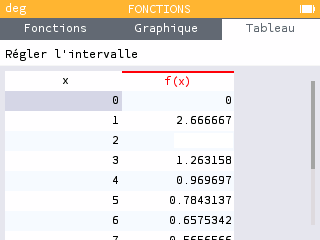
\includegraphics[width=8cm]{evaluation_10_sujet_B_numworks.png}
	\item \hspace*{-1cm}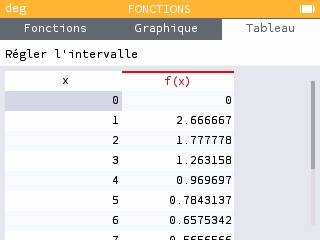
\includegraphics[width=8cm]{evaluation_10_sujet_B_numworks_bis.png}
      \end{itemize}
    \end{multicols}
    \begin{enumerate}
      \item Dans les réglages de la calculatrice, quel pas a-t-on choisi ?\rep{4}
      \item Quel est le nombre manquant ?\rep{4}
    \end{enumerate}
  \item Dans le repère ci-dessous, tracer la courbe représentative de $f$.
    \begin{center}
      \newrgbcolor{ffvvqq}{1. 0.3333333333333333 0.}
      \psset{xunit=0.7cm,yunit=0.7cm,algebraic=true,dimen=middle,dotstyle=o,dotsize=5pt 0,linewidth=1.pt,arrowsize=3pt 2,arrowinset=0.25}
      \begin{pspicture*}(-9.,-5.)(9.,5.)
	\multips(0,-5)(0,1.0){11}{\psline[linestyle=dashed,linecap=1,dash=1.5pt 1.5pt,linewidth=0.4pt,linecolor=lightgray]{c-c}(-9.,0)(9.,0)}
	\multips(-9,0)(1.0,0){19}{\psline[linestyle=dashed,linecap=1,dash=1.5pt 1.5pt,linewidth=0.4pt,linecolor=lightgray]{c-c}(0,-5.)(0,5.)}
	\psaxes[labelFontSize=\scriptstyle,xAxis=true,yAxis=true,Dx=1.,Dy=1.,ticksize=-2pt 0,subticks=2]{->}(0,0)(-9.,-5.)(9.,5.)
	%\psplot[linewidth=1.pt,linecolor=ffvvqq,plotpoints=200]{-9.0}{9.0}{8*x/(2*x^(2.0)+1.0)}
      \end{pspicture*}
    \end{center}
  \item Le point $A(4;1)$ appartient-il à la courbe de $f$ ?\rep{4}
  \item Même question avec le point $B\left(-6;-\dfrac{48}{73}\right)$.\rep{4}
\end{enumerate}
\end{document}
